%!TeX root=../tese.tex
%("dica" para o editor de texto: este arquivo é parte de um documento maior)
% para saber mais: https://tex.stackexchange.com/q/78101/183146

%% ------------------------------------------------------------------------- %%
\chapter{Relação entre as delimitações de Wilber}
\label{cap:relacao-wilber}

Nesta capítulo estabeleceremos uma relação entre a delimitação da alternância e a delimitação do funil. Faremos isso por meio de um argumento geométrico a partir de uma caracterização nova de z-retângulos proposta por Lecomte e Weistein \cite{new_boundaries}.

\section{Rotação e inversão de conjuntos de pontos}
Pouco se sabe sobre a relação entre a delimitação da alternância e do funil para sequências de acessos arbitrárias. Assim, neste capítulo consideraremos apenas sequências de acessos sem repetições.

Seja $P$ um conjunto de pontos. Definimos a inversão temporal de um ponto $p \in P$ como $\widebar{p} = (p.x,-p.y)$. Definimos a inversão temporal de um conjunto de pontos $P$ como $\widebar{P} = \{\widebar{p} \mid p \in P\}$. Na prática, a inversão temporal de um conjunto de pontos é o conjunto resultante do espelhamento de cada um dos seus pontos em relação ao eixo das abscissas. Veja a Figura~\ref{fig:inversao}.

\begin{figure}
    \centering
    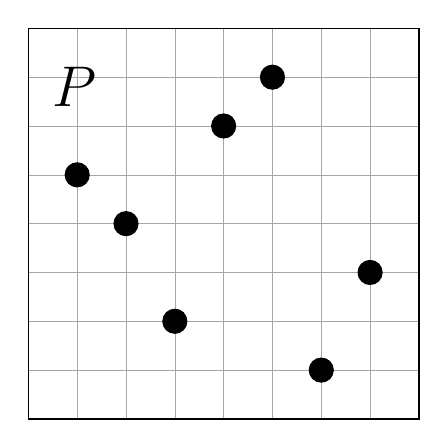
\begin{tikzpicture}[scale=0.62]
        \draw[very thin, gray!70] (0,0) grid (8,8);        
        \filldraw[black] (6,1) circle (7pt);
        \filldraw[black] (3,2) circle (7pt);
        \filldraw[black] (7,3) circle (7pt);
        \filldraw[black] (2,4) circle (7pt);
        \filldraw[black] (1,5) circle (7pt);
        \filldraw[black] (4,6) circle (7pt);
        \filldraw[black] (5,7) circle (7pt);
        \draw[black, line width=0.5pt] (0,0) rectangle (8,8);

        \node[anchor=south west] at (0.3,6.2) {\huge$P$};
    \end{tikzpicture}
    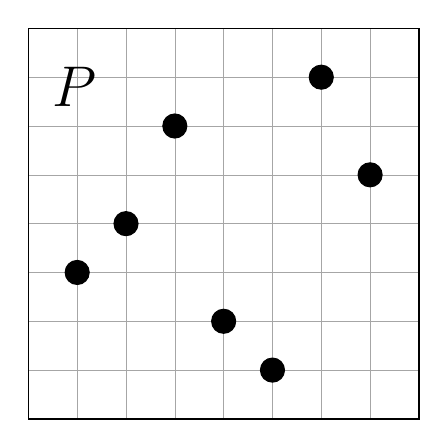
\begin{tikzpicture}[scale=0.62]
        \draw[very thin, gray!70] (0,0) grid (8,8);
        \filldraw[black] (5,1) circle (7pt);
        \filldraw[black] (4,2) circle (7pt);
        \filldraw[black] (1,3) circle (7pt);
        \filldraw[black] (2,4) circle (7pt);
        \filldraw[black] (7,5) circle (7pt);
        \filldraw[black] (3,6) circle (7pt);
        \filldraw[black] (6,7) circle (7pt);
        \draw[black, line width=0.5pt] (0,0) rectangle (8,8);

        \node[anchor=south west] at (0.3,6.2) {\huge$\widebar{P}$};
    \end{tikzpicture}
    \caption{À esquerda, um conjunto $P$ de pontos. À direita, a sua inversão temporal $\protect\widebar{P}$.}
\label{fig:inversao}
\end{figure}

Analogamente, definimos a rotação de 90° em sentido anti-horário de um ponto $p \in P$ como $p^{\perp} = (-p.y,p.x)$. A rotação de 90° em sentido anti-horário de um conjunto de pontos $P$ é definida por $P^{\perp} = \{p^{\perp} \mid p \in P\}$. Veja a figura~\ref{fig:rotacao}.

\begin{figure}
    \centering
    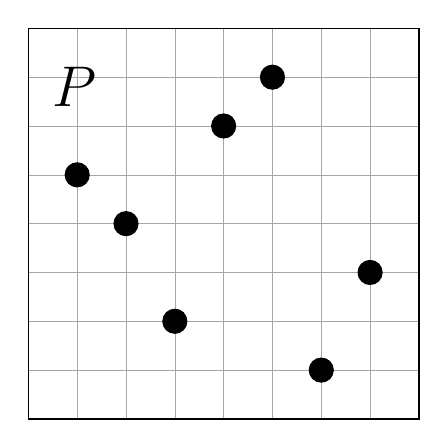
\begin{tikzpicture}[scale=0.62]
        \draw[very thin, gray!70] (0,0) grid (8,8);        
        \filldraw[black] (6,1) circle (7pt);
        \filldraw[black] (3,2) circle (7pt);
        \filldraw[black] (7,3) circle (7pt);
        \filldraw[black] (2,4) circle (7pt);
        \filldraw[black] (1,5) circle (7pt);
        \filldraw[black] (4,6) circle (7pt);
        \filldraw[black] (5,7) circle (7pt);
        \draw[black, line width=0.5pt] (0,0) rectangle (8,8);

        \node[anchor=south west] at (0.3,6.2) {\huge$P$};
    \end{tikzpicture}
    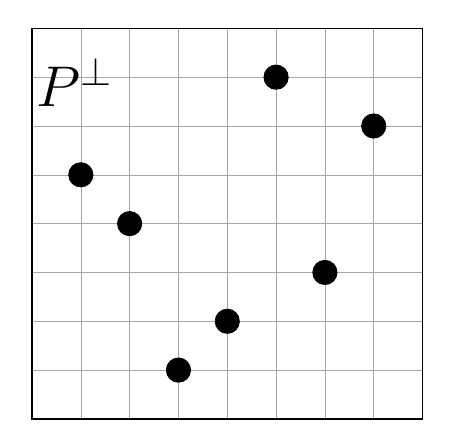
\begin{tikzpicture}[scale=0.62]
        \draw[very thin, gray!70] (0,0) grid (8,8);
        \filldraw[black] (7,6) circle (7pt);
        \filldraw[black] (6,3) circle (7pt);
        \filldraw[black] (5,7) circle (7pt);
        \filldraw[black] (4,2) circle (7pt);
        \filldraw[black] (3,1) circle (7pt);
        \filldraw[black] (2,4) circle (7pt);
        \filldraw[black] (1,5) circle (7pt);
        \draw[black, line width=0.5pt] (0,0) rectangle (8,8);

        \node[anchor=south west] at (-0.1,6.2) {\huge$P^{\perp}$};
    \end{tikzpicture}
    \caption{À esquerda, o conjunto de pontos $P_X$ relativo à sequência $X =(6,3,5,4,2,1,7)$ de acessos. À direita, a inversão temporal de $P_X$.}
\label{fig:rotacao}
\end{figure}

\section{Relação da alternância com o funil e a inversão temporal}

Primeiramente, é necessário entender como a delimitação da alternância para um conjunto $P$ de pontos está relacionada com a delimitação do funil de $P$ e de $\widebar{P}$.

\begin{lemma} \label{lemma:relacao-alt-com-funil}
    Seja $P_X$ a visão geométrica de uma sequência de acessos sem repetições e $\cT$ uma árvore de referência em relação a $P_X$. Então, $\Funil(P_X) +  \Funil(\widebar{P_X}) \geq  \Alt_{\cT}(P_X)$.
\end{lemma}

\begin{proof}
    Provaremos, por indução em $k$, que toda árvore $\cT$ com $k$ nós satisfaz a desigualdade do lema.

    Para $k = 1$, a árvore de referência $\cT$ possui um único nó. Assim, \Alt$_{\cT}(P_X) = 0$ e a desigualdade é válida trivialmente.

    Suponha agora que $k > 1$ e que a propriedade vale para toda árvore com menos que $k$ nós. Sejam $\cT_{E}$ e $\cT_{D}$ respectivamente a subárvore esquerda e a subárvore direita da raiz de $\cT$. Sejam $P_E = \{p \in P_X \mid p.x \in \cT_E\}$ e $P_D = \{p \in P_X \mid p.x \in \cT_D\}$. Pela hipótese de indução, temos
    \begin{center}
    $\Funil(P_E) +  \Funil(\widebar{P_E}) \geq  \Alt_{\cT_E}(P_E)$ \mbox{e} $\Funil(P_D) +  \Funil(\widebar{P_D}) \geq  \Alt_{\cT_D}(P_D)$.
    \end{center}
    Assim, temos que
    \begin{align}
        \Alt_{\cT}(P_X) &= a(P_X,\cT) + \Alt_{\cT_E}(P_X) + \Alt_{\cT_D}(P_X), \notag \\
        &\leq a(P_X,\cT) + \Funil(P_E) +  \Funil(\widebar{P_E}) + \Funil(P_D) +  \Funil(\widebar{P_D}). \label{eq:inicio}
    \end{align}

    Agora, é necessário entender como a delimitação do funil é afetada pela inversão temporal do conjunto de pontos.
    Seja $p$ um ponto de $P_X$. Lembre-se das definições de $F_E$,$F_D$ e $f$ da Seção~\ref{seção:funil}.
    Mostraremos que se $p \in P_E$, então $f(P_X,p) \geq f(P_E,p)$ e $f(\widebar{P_X},\widebar{p}) \geq f(\widebar{P_E},\widebar{p})$. De maneira simétrica, se $p \in P_D$ então $f(P_X,p) \geq f(P_D,p)$ e $f(\widebar{P_X},\widebar{p}) \geq f(\widebar{P_D},\widebar{p})$.

    Suponha que $p \in P_E$. Como $p$ pertence a $P_E$, então todos os pontos a esquerda de $p$ também pertencem a $P_E$, ou seja, $F_E(P_E,p) = F_E(P_X,p)$. Além disso, todos os pontos que pertencem a $P_E$ e estão à direita de $p$ pertencem ao lado direito do funil de $p$ tanto em relação a $P_E$ quanto em relação a $P_X$, ou seja, $F_D(P_E,p) \subseteq F_D(P_X,p)$. Veja a Figura~\ref{fig:funis}. Assim, $mix(F_E(P_E,p).y,F_D(P_E,p).y)$ é uma subsequência de $mix(F_E(P_X,p).y,F_D(P_X,p).y)$, logo 
    \begin{center}
        $blocos(mix(F_E(P_E,p), F_D(P_E,p))) \leq blocos(mix(F_E(P_X,p), F_D(P_X,p)))$ \mbox{e}
        $f(P_E,p) \leq f(P_X,p)$.
    \end{center}
    Por simetria, o argumento vale para os outros casos.
    \begin{figure}
        \centering
        \includegraphics[scale=1.04]{imagens/funis.pdf}
        \caption{À esquerda, uma árvore de referência $\cT$ em relação à visão geométrica da sequência de acessos $X = (4,6,2,5,1,7,3)$. Note que $P_E = \{1,2,3,4\}$. À direita, quatro conjuntos de pontos. Denotemos por $p$ o ponto $(3,7)$ destacado de azul. Os conjuntos de pontos vermelhos de cima representam respectivamente $F_E(P_E,p)$ e $F_D(P_E,p)$. Os conjuntos de pontos vermelhos embaixo representam respectivamente $F_E(P_X,p)$ e $F_D(P_X,p)$. Perceba que $F_E(P_E,p) = F_E(P_X,p)$ e $F_D(P_E,p) \subseteq F_D(P_X,p)$.}
    \label{fig:funis}
    \end{figure}

    Ao somarmos $f(P_X,p)$ para todo $p \in P_X$, temos
    \begin{align}
        \Funil(P_X) &= \sum_{p \, \in \, P_X}f(P_X,p), \notag\\
        &\geq \sum_{p \, \in \, P_E}f(P_E,p) + \sum_{p \, \in \, P_D}f(P_D,p), \notag \\
        &= \Funil(P_E) + \Funil(P_D). \label{eq:funil}
    \end{align}

    Analogamente, para a inversão temporal, temos que
    \begin{align}
        \Funil(\widebar{P_X}) &= \sum_{p \, \in \, P_X}f(\widebar{P_X},\widebar{p}), \notag\\
        &\geq \sum_{p \, \in \, P_E}f(\widebar{P_E},\widebar{p}) + \sum_{p \, \in \, P_D}f(\widebar{P_D},\widebar{p}), \notag \\
        &= \Funil(\widebar{P_E}) + \Funil(\widebar{P_D}). \label{eq:funil_barra}
    \end{align}

    Combinando as Equações (\ref{eq:inicio}), (\ref{eq:funil}) e (\ref{eq:funil_barra}), concluímos que
    \begin{align}
        \Funil(P_X) + \Funil(\widebar{P_X}) &\geq \Funil(P_E) + \Funil(P_D) + \Funil(\widebar{P_E}) + \Funil(\widebar{P_D}), \notag \\
        &\geq \Alt_{\cT}(P_X) - a(P_X,\cT).
        \label{eq:medio}
    \end{align}

    Para terminar a indução, basta retirar o termo $a(P_X,\cT)$ da Equação~(\ref{eq:medio}). Para isso, precisamos entender como a intercalação é afetada quando consideramos $P_X$ e apenas um dos conjuntos $P_E$, $P_D$, $\widebar{P_E}$ e $\widebar{P_D}$.

    Vamos definir quatro propriedades que serão utilizadas a seguir:
    \begin{enumerate}[label=(\alph*)]  % Usando letras com parênteses
        \item $p \in \cT_E$ e $f(P_X,p) \geq f(P_E,p) + 1$,
        \item $p \in \cT_E$ e $f(\widebar{P_X},\widebar{p}) \geq f(\widebar{P_E},\widebar{p}) + 1$,
        \item $p \in \cT_D$ e $f(P_X,p) \geq f(P_D,p) + 1$,
        \item $p \in \cT_D$ e $f(\widebar{P_X},\widebar{p}) \geq f(\widebar{P_D},\widebar{p}) + 1$.
    \end{enumerate}

    Vamos enumerar os pontos de $P_X$ de maneira cronológica com $y$-coordenada crescente como $p_1,\ldots,p_m$ e dividiremos a análise em seis casos.
    Como $a(P_X,\cT) = \emph{intercala}(P_E.y,P_D.y)$ e $P_E$ e $P_D$ não são vazios pois $k > 1$, então $a(P_X,\cT) \geq 2$. Assim, quando analisamos cronologicamente os pontos de $P_X$, há $a(P_X,\cT) - 1 \geq 1$ alternâncias entre pontos de $P_E$ e pontos de $P_D$. Logo, há exatamente $a(P_X,\cT) - 2$ pares de pontos consecutivos em relação ao lado esquerdo ou direito do seu funil que possuem diferença no eixo $y$ de mais de uma unidade. Formalmente, há exatamente $a(P_X,\cT) - 2$ pares $(i,j)$ de índices tais que $i + 1 < j$ para os quais 
    \begin{center}
        caso 1: $p_i,p_j \in P_E$ e $p_{i+1},\ldots,p_{j-1} \in P_D$,\\
        caso 2: $p_i,p_j \in P_D$ e $p_{i+1},\ldots,p_{j-1} \in P_E$.
    \end{center}

    Além disso, há um índice $i^{*} > 1$ que representa o primeiro ponto do lado do funil que não possui o ponto mais baixo de $P_X$, ou seja,
    \begin{center}
        caso 3: $p_{i^{*}} \in P_E$ e $p_1,\ldots,p_{i^{*}-1} \in P_D$,\\
        caso 4: $p_{i^{*}}  \in P_D$ e $p_1,\ldots,p_{i^{*}-1} \in P_E$.
    \end{center}

    Por último, há um índice $j^{*} < m$ que representa o último ponto do lado do funil que não possui o ponto mais alto de $P_X$, ou seja,
    \begin{center}
        caso 5: $p_{j^{*}} \in P_E$ e $p_{j^{*} + 1},\ldots,p_m \in P_D$,\\
        caso 6: $p_{j^{*}}  \in P_D$ e $p_{j^{*} + 1},\ldots,p_m \in P_E$.
    \end{center} 

    \begin{figure}
        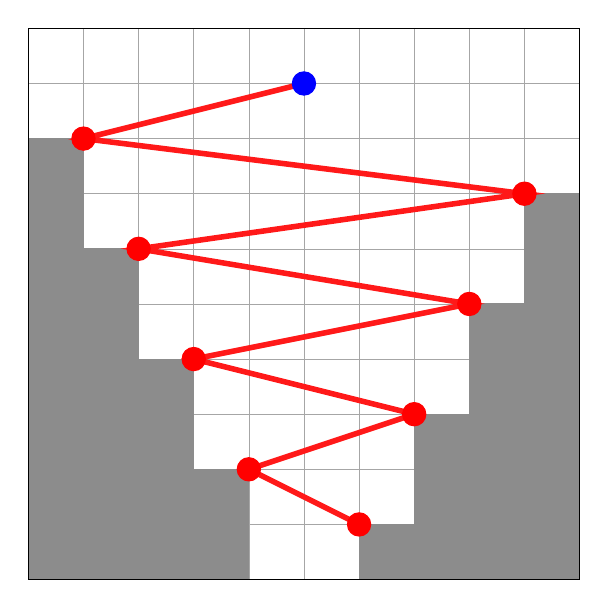
\begin{tikzpicture}[scale=0.7]
            \draw[very thin, gray!70] (0,0) grid (10,10);
            
            \draw[fill=gray!90, gray!90] (0,0) rectangle (1,8);
            \draw[fill=gray!90, gray!90] (0,0) rectangle (2,6);
            \draw[fill=gray!90, gray!90] (0,0) rectangle (3,4);
            \draw[fill=gray!90, gray!90] (0,0) rectangle (4,2);
            \draw[fill=gray!90, gray!90] (10,0) rectangle (9,7);
            \draw[fill=gray!90, gray!90] (10,0) rectangle (8,5);
            \draw[fill=gray!90, gray!90] (10,0) rectangle (7,3);
            \draw[fill=gray!90, gray!90] (10,0) rectangle (6,1);
    
              
            \draw[red!90, line width=2pt] (5,9) -- (1,8) -- (9,7) -- (2,6) -- (8,5) -- (3,4) -- (7,3) -- (4,2) -- (6,1);  

            \filldraw[red] (6,1) circle (6pt);
            \filldraw[red] (4,2) circle (6pt);
            \filldraw[red] (7,3) circle (6pt);
            \filldraw[red] (3,4) circle (6pt);
            \filldraw[red] (8,5) circle (6pt);
            \filldraw[red] (2,6) circle (6pt);
            \filldraw[red] (9,7) circle (6pt);
            \filldraw[red] (1,8) circle (6pt);
            \filldraw[blue] (5,9) circle (6pt);
    
            \draw[black, line width=0.5pt] (0,0) rectangle (10,10);
        \end{tikzpicture}
        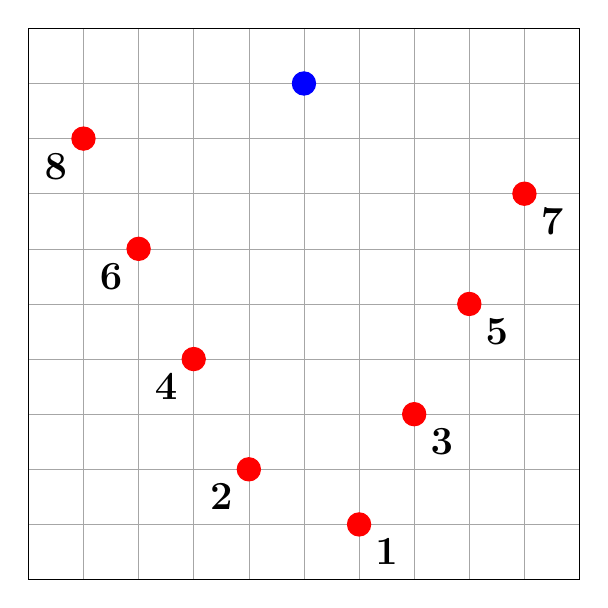
\begin{tikzpicture}[scale=0.7]
            \draw[very thin, gray!70] (0,0) grid (10,10);       
              
            %\draw[red!90, line width=2pt] (5,9) -- (1,8) -- (9,7) -- (2,6) -- (8,5) -- (3,4) -- (7,3) -- (4,2) -- (6,1);  

            \filldraw[red] (6,1) circle (6pt);
            \filldraw[red] (4,2) circle (6pt);
            \filldraw[red] (7,3) circle (6pt);
            \filldraw[red] (3,4) circle (6pt);
            \filldraw[red] (8,5) circle (6pt);
            \filldraw[red] (2,6) circle (6pt);
            \filldraw[red] (9,7) circle (6pt);
            \filldraw[red] (1,8) circle (6pt);
            \filldraw[blue] (5,9) circle (6pt);

            \node at (6.5,0.5) {\textbf{\Large 1}};
            \node at (7.5,2.5) {\textbf{\Large 3}};
            \node at (8.5,4.5) {\textbf{\Large 5}};
            \node at (9.5,6.5) {\textbf{\Large 7}};
            \node at (3.5,1.5) {\textbf{\Large 2}};
            \node at (2.5,3.5) {\textbf{\Large 4}};
            \node at (1.5,5.5) {\textbf{\Large 6}};
            \node at (0.5,7.5) {\textbf{\Large 8}};
    
            \draw[black, line width=0.5pt] (0,0) rectangle (10,10);
        \end{tikzpicture}
        \caption{À esquerda, está destacada a delimitação do funil para o ponto $(5,9)$ da visão geométrica da sequência $X = (6,4,7,3,8,2,9,1,5)$ de acessos e, à direita, estão numerados de $1$ a $8$ os pontos do funil deste ponto. Perceba que os pares de índices $(2,4),(4,6),(6,8)$ representam o caso 1. Os pares de índices $(1,3),(3,5),(5,7)$ representam o caso 2. Além disso, o caso 3 acontece com índice $i^{*} = 2$ e também o caso 6 com índice $j^{*} = 7$.}
    \label{fig:espelhamento-de-funil-inicial}
    \end{figure}

    Assim, percebemos que os casos 3 e 4 não ocorrem simultaneamente, assim como os casos 5 e 6. Logo, sempre acontece exatamente 1 caso de cada um desses pares. Como os primeiros dois casos acontecem $a(P_X,\cT) - 2$ vezes, então somados temos $a(P_X,\cT)$ ocorrências de todos os seis casos. Veja a Figura~\ref{fig:espelhamento-de-funil-inicial}.

    Cada caso desses implica em uma das propriedades dentre (a), (b), (c) e (d). Mais precisamente,

    
    \begin{tabular}{l}
        caso 1 implica que $p_j$ possui a propriedade (a) ou $p_i$ possui a propriedade (b),\\
        caso 2 implica que $p_j$ possui a propriedade (c) ou $p_i$ possui a propriedade (d),\\
        caso 3 implica que $p_{i^{*}}$ possui a propriedade (a),\\
        caso 4 implica que $p_{i^{*}}$ possui a propriedade (c),\\
        caso 5 implica que $p_{j^{*}}$ possui a propriedade (b),\\
        caso 6 implica que $p_{j^{*}}$ possui a propriedade (d).
    \end{tabular}
    
    Provaremos a afirmação para o caso 1 e para o caso 3. O restante dos casos é análogo.

    Para o caso 1, se $p_i.x < p_j.x$, então vamos provar que $f(P_X,p_j) \geq f(P_E,p_j) + 1$. Veja que $p_i$ está no lado esquerdo do funil de $p_j$ tanto em relação a $P_X$ quanto em relação a $P_E$. Mas, em relação a $P_X$, $p_{j-1}$ é um ponto adicional do funil de $p_j$ quando comparado com o funil de $p_j$ em relação a $P_E$. Assim, $f(P_X,p_j) \geq f(P_E,p_j) + 1$.
    Se $p_i.x > p_j.x$, é possível usar o mesmo argumento para $\widebar{P_X}$ e $\widebar{P_E}$ analisando o ponto $p_i$ e concluir que, $f(\widebar{P_X},\widebar{p_i}) \geq f(\widebar{P_E},\widebar{p_i}) + 1$.

    Para provar o caso 3, basta perceber que ambos os funis de $p_{i^{*}}$ em relação a $P_E$ são vazios por não existirem pontos abaixo de $p_{i^{*}}$ que pertença a $P_E$. Já em relação a $P_X$, o lado direito do funil de $p_{i^{*}}$ possui pelo menos o ponto $p_{i^{*} - 1}$. Logo, $f(P,p_{i^{*}}) \geq 1 = f(P_E,p_{i^{*}}) + 1$, já que $f(P_E,p_{i^{*}}) = 0$. 

    Assim, é possível recombinar as Equações (\ref{eq:inicio}), (\ref{eq:funil}) e (\ref{eq:funil_barra}), e concluir que na verdade
    \begin{align*}
        \Funil(P) + \Funil(\widebar{P}) &\geq \Funil(P_E) + \Funil(P_D) + \Funil(\widebar{P_E}) + \Funil(\widebar{P_D}) + a(P_X,\cT), \notag \\
        &\geq \Alt_{\cT}(P_X).
    \end{align*}

    Assim, terminamos a prova indutiva.
\end{proof}

Apesar do Lema~\ref{lemma:relacao-alt-com-funil} relacionar as duas delimitações com a ajuda da inversão temporal de $P_X$, ele não é de grande utilidade isolada, pois não sabemos como \Funil$(P)$ e \Funil$(\widebar{P})$ se relacionam.

\section{Relação do funil e sua inversão temporal}

Precisamos entender agora como as transformações geométricas afetam a delimitação do funil. A delimitação não é afetada por espelhamentos no eixo $y$. Isso porque o número de intercalações entre os funis se mantém igual e assim a função \emph{intercala} para cada ponto não tem seu valor alterado. Veja a Figura~\ref{fig:espelhamento-de-funil}.

\begin{figure}
    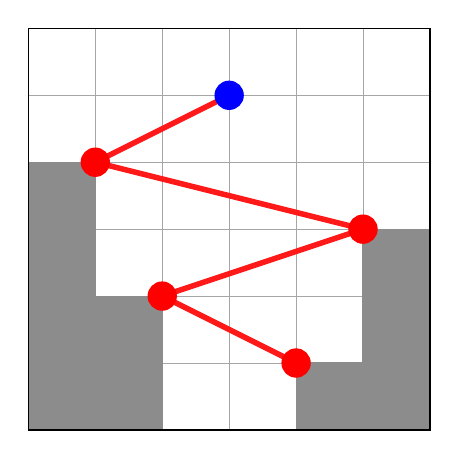
\begin{tikzpicture}[scale=0.85]
        \draw[very thin, gray!70] (0,0) grid (6,6);
        
        \draw[fill=gray!90, gray!90] (6,0) rectangle (6,5);
        \draw[fill=gray!90, gray!90] (6,0) rectangle (5,3);
        \draw[fill=gray!90, gray!90] (6,0) rectangle (4,1);
        \draw[fill=gray!90, gray!90] (0,0) rectangle (2,2);
        \draw[fill=gray!90, gray!90] (0,0) rectangle (1,4);

          
        \draw[red!90, line width=2pt] (3,5) -- (1,4) -- (5,3) -- (2,2) -- (4,1);  

        \filldraw[red] (4,1) circle (6pt);
        \filldraw[red] (2,2) circle (6pt);
        \filldraw[red] (5,3) circle (6pt);
        \filldraw[red] (1,4) circle (6pt);
        \filldraw[blue] (3,5) circle (6pt);

        \draw[black, line width=0.5pt] (0,0) rectangle (6,6);
    \end{tikzpicture}
    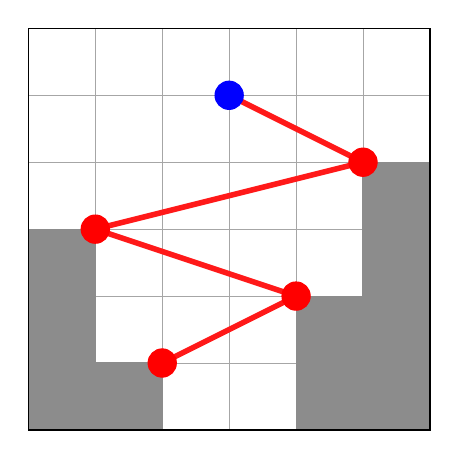
\begin{tikzpicture}[scale=0.85]
        \draw[very thin, gray!70] (0,0) grid (6,6);
        
        \draw[fill=gray!90, gray!90] (0,0) rectangle (0,5);
        \draw[fill=gray!90, gray!90] (0,0) rectangle (1,3);
        \draw[fill=gray!90, gray!90] (0,0) rectangle (2,1);
        \draw[fill=gray!90, gray!90] (6,0) rectangle (4,2);
        \draw[fill=gray!90, gray!90] (6,0) rectangle (5,4);

          
        \draw[red!90, line width=2pt] (3,5) -- (5,4) -- (1,3) -- (4,2) -- (2,1);  

        \filldraw[red] (2,1) circle (6pt);
        \filldraw[red] (4,2) circle (6pt);
        \filldraw[red] (1,3) circle (6pt);
        \filldraw[red] (5,4) circle (6pt);
        \filldraw[blue] (3,5) circle (6pt);

        \draw[black, line width=0.5pt] (0,0) rectangle (6,6);
    \end{tikzpicture}
    \caption{À esquerda, está destacado o funil do ponto azul. À direita, está destacado o funil do mesmo ponto no conjunto inicial espelhado em relação ao eixo $y$. Em ambos os casos há o mesmo número de alternâncias entre o lado esquerdo e o direito do funil do ponto azul.}
\label{fig:espelhamento-de-funil}
\end{figure}

Porém o valor da delimitação pode se alterar com a inversão temporal. Veja a Figura~\ref{fig:espelhamento-de-funil-2}.

\begin{figure}
    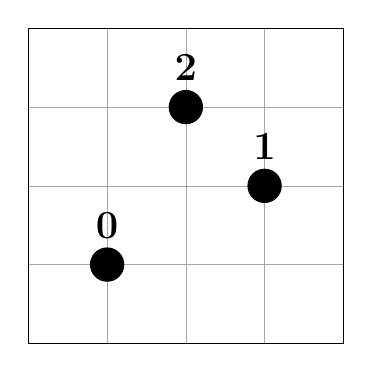
\begin{tikzpicture}[scale=1]
        \draw[very thin, gray!70] (0,0) grid (4,4);

        \filldraw[black] (1,1) circle (6pt);
        \filldraw[black] (3,2) circle (6pt);
        \filldraw[black] (2,3) circle (6pt);

        \node at (1,1.5) {\textbf{\Large 0}};
        \node at (3,2.5) {\textbf{\Large 1}};
        \node at (2,3.5) {\textbf{\Large 2}};

        \draw[black, line width=0.5pt] (0,0) rectangle (4,4);
    \end{tikzpicture}
    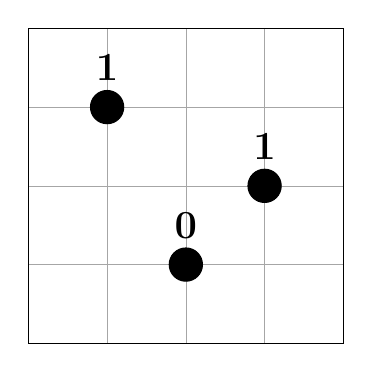
\begin{tikzpicture}[scale=1]
        \draw[very thin, gray!70] (0,0) grid (4,4);

        \filldraw[black] (2,1) circle (6pt);
        \filldraw[black] (3,2) circle (6pt);
        \filldraw[black] (1,3) circle (6pt);

        \node at (2,1.5) {\textbf{\Large 0}};
        \node at (3,2.5) {\textbf{\Large 1}};
        \node at (1,3.5) {\textbf{\Large 1}};

        \draw[black, line width=0.5pt] (0,0) rectangle (4,4);
    \end{tikzpicture}
    \caption{À esquerda, a visão geométrica da sequência $X = (1,3,2)$ de acessos. À direita, a inversão temporal de $P_X$. Acima de cada ponto está o valor de sua delimitação do funil. Assim, \Funil$(P_X) = 0 + 1 + 2 = 3$, enquanto que \Funil$(\protect \widebar{P_X}) = 0 + 1 + 1 = 2$.}
\label{fig:espelhamento-de-funil-2}
\end{figure}

Assim, a princípio \Funil$(P)$ e \Funil$(\widebar{P})$ podem ter valores muito diferentes. Para entender essa relação, precisamos caracterizar a delimitação do funil de maneira invariante em relação a rotações de 90°. 

Para um conjunto $P$ de pontos, chamamos de \textit{z-retângulo} qualquer sequência de quatro pontos $(p,q,r,s) \in P^4$ com as seguintes propriedades: $q.x < p.x < r.x < s.x$, \ $r.y < q.y < s.y < p.y$ e $P \cap [q.x,s.x] \times [r.y,p.y]  = \{p,q,r,s\}$. Na prática, um z-retângulo é uma sequência de 4 pontos de $P$ que cronologicamente possuem $x$-coordenadas relativas 3,1,4,2 e o retângulo que contém todos os quatro pontos em seu perímetro não possui nenhum outro ponto de $P$. Veja a Figura~\ref{fig:z-retangulo-isolado}. Definimos por \textit{zRet(P)} o número de z-retângulos de $P$.

\begin{figure}
    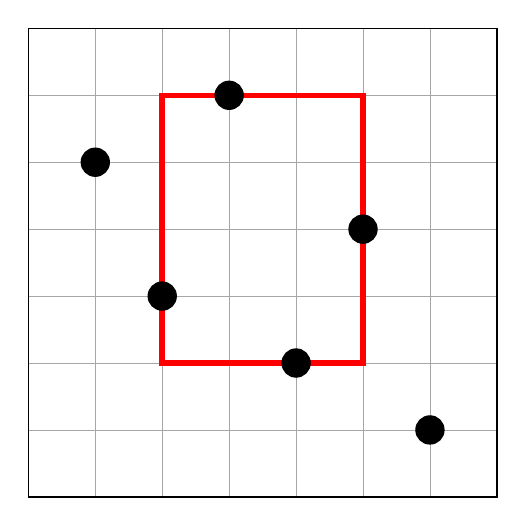
\begin{tikzpicture}[scale=0.85]
        \draw[very thin, gray!70] (0,0) grid (7,7);

        \draw[red, line width=0.07cm] (2,2) rectangle (5,6);

        \filldraw[black] (6,1) circle (6pt);
        \filldraw[black] (4,2) circle (6pt);
        \filldraw[black] (2,3) circle (6pt);
        \filldraw[black] (5,4) circle (6pt);
        \filldraw[black] (1,5) circle (6pt);
        \filldraw[black] (3,6) circle (6pt);

        \draw[black, line width=0.5pt] (0,0) rectangle (7,7);
    \end{tikzpicture}
    \caption{O único z-retângulo da visão geométrica da sequência $X = (6,4,2,5,1,3)$ de acessos.}
\label{fig:z-retangulo-isolado}
\end{figure}

\begin{lemma}\label{lemma:p-inversivel}
    Para qualquer conjunto $P$ de pontos, $zRet(P) = zRet(P^{\perp})$.
\end{lemma}

\begin{proof}
    Ao rotacionar $P$, o z-retângulo $(p,q,r,s)$ de $P$ se tornará o z-retângulo $(s^{\perp},p^{\perp},q^{\perp},r^{\perp})$ em $P^{\perp}$. Uma maneira simples de perceber esse fenômeno é rotacionar a Figura~\ref{fig:z-retangulo-isolado}. Perceba que a $x$-coordenada relativa 3,1,4,2 é invariante em relação a rotações de 90°.
\end{proof}

\begin{lemma}
    Para qualquer ponto $p$ de um conjunto $P$ de pontos, existem $\lfloor f(P,p)/2 \rfloor - 1$ z-retângulos formados por $p$ e três de pontos de seu funil.
\end{lemma}

\begin{proof} \label{lema:passo-intermediario}
    Para um ponto $p \in P$ com $l$ pontos em seu funil, enumeremos os pontos de seu funil de maneira cronológica $(a_1,a_2,\ldots,a_l)$, onde $a_1.y < a_2.y < \cdots < a_l.y$. Suponha que $f(P,p) \geq 4$, caso contrário a delimitação é imediata.

    Chamamos um par $(i,j)$ de índices de \textit{separador esquerdo} se $i + 1 < j$, $a_i.x > p.x$, $a_j.x > p.x$ e para todo $k$ com $i < k < j$, $a_k.x < p.x$. Em outras palavras, chamamos um par $(i,j)$ de índices de separador esquerdo se ambos os pontos $a_i$ e $a_j$ estão à direita de $p$ e todos os pontos com índice $k$ entre $i$ e $j$ estão à esquerda de $p$.

    Sabemos que há $f(P,p)$ intercalações entre o lado esquerdo e o lado direito do funil de $p$. Como os funis de $p$ se alternam $f(P,p) -1$ vezes, então, no pior dos casos onde as intercalações se iniciam e terminam no lado esquerdo do funil de $p$, existem  $\lfloor f(P,p)/2 \rfloor - 1$ pares separadores de índices de $p$. Veja a Figura~\ref{fig:bound-z-rets}.

    %figure!
    \begin{figure}
        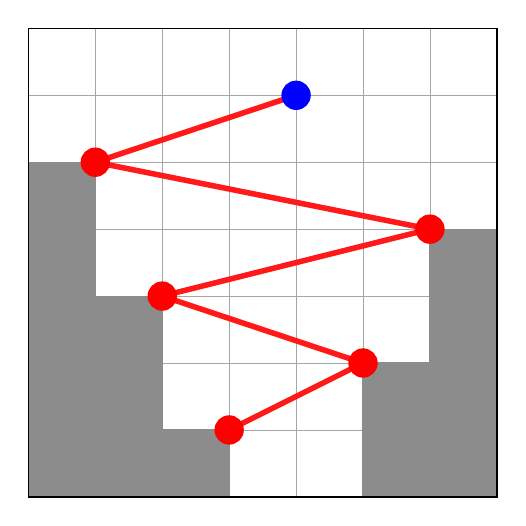
\begin{tikzpicture}[scale=0.85]
            \draw[very thin, gray!70] (0,0) grid (7,7);  
            
            \draw[fill=gray!90, gray!90] (0,0) rectangle (3,1);
            \draw[fill=gray!90, gray!90] (0,0) rectangle (2,3);
            \draw[fill=gray!90, gray!90] (0,0) rectangle (1,5);
            \draw[fill=gray!90, gray!90] (7,0) rectangle (5,2);
            \draw[fill=gray!90, gray!90] (7,0) rectangle (6,4);
              
            \draw[red!90, line width=2pt] (3,1) -- (5,2) -- (2,3) -- (6,4) -- (1,5) -- (4,6);  
    
            \filldraw[red] (3,1) circle (6pt);
            \filldraw[red] (5,2) circle (6pt);
            \filldraw[red] (2,3) circle (6pt);
            \filldraw[red] (6,4) circle (6pt);
            \filldraw[red] (1,5) circle (6pt);
            \filldraw[blue] (4,6) circle (6pt);
    
            \draw[black, line width=0.5pt] (0,0) rectangle (7,7);
        \end{tikzpicture}
        \caption{Em azul, o ponto $p = (4,6)$ do conjunto $P$ de pontos. Em vermelho, os pontos de seu funil e suas intercalações. Perceba que $f(P,p) = 5$. Os pontos mais alto e mais baixo do funil de $p$ pertencem ao lado esquerdo de seu funil e há apenas $\lfloor f(P,p)/2 \rfloor - 1 = 1$ pares separadores esquerdos de índices.}
    \label{fig:bound-z-rets}
    \end{figure}

    Assim, para cada par separador esquerdo de índices $(i,j)$, note que os pontos $(p,a_{i+1},a_i,a_j)$ caracterizam um z-retângulo. Pela ordem dos índices, é fácil perceber que $p.y > a_j.y > a_{i+1}.y > a_i.y$. Como as $x$-coordenadas dos pontos do lado direito do funil estão em ordem cronológica crescente, então sabemos que $a_j.x > a_i.x > p.x > a_{i+1}.x$. Assim, concluímos que as posições relativas estão corretas, formando um z-retângulo.

    Por fim, é necessário garantir que $P \cap [a_{i+1}.x,a_j.x] \times [a_i.y,p.y] = \{p,a_i,a_{i+1},a_j\}$, ou seja, não há nenhum outro ponto de $P$ dentro da área delimitada pelo retângulo que possui os pontos $p$, $a_i$, $a_{i+1}$ e $a_j$ em seu perímetro. Por $a_i$ e $a_j$ serem pontos consecutivos do lado direito do funil de $p$, sabemos que não há nenhum ponto no lado direito do funil de $p$ com $y$-coordenada entre $a_i.y$ e $a_j.y$. Como os pontos do lado esquerdo do funil de $p$ possuem $x$-coordenada cronologicamente decrescente e não existe nenhum ponto do funil de $p$ com $y$-coordenada entre $a_i.y$ e $a_{i+1}.y$, então conclui-se que não há nenhum ponto $q \in P \setminus \{p,a_i,a_{i+1},a_j\}$, no $\{a_i,a_{i+1}\}$-retângulo, no $\{a_j,a_{i+1}\}$-retângulo ou no $\{p,a_{i+1}\}$-retângulo. Por fim, pelos pontos do lado direito do funil possuírem $x$-coordenada cronologicamente crescente, então também não há um ponto $q \in P \setminus \{p,a_j\}$ no $\{p,a_j\}$-retângulo. Veja a Figura~\ref{fig:representacao-areas}. 

    %\fill[pattern=vertical lines] (A) -- (C) -- (end) -- (start) -- cycle;
    \begin{figure}
        \begin{tikzpicture}[scale=0.85]
            % Grade de fundo
            \draw[very thin, gray!70] (0,0) grid (5,5);  
            \draw[red,line width=0.07cm] (1,1) rectangle (4,4);

            \fill[pattern=north west lines] (3,1) -- (4,1) -- (4,3) -- (3,3) -- cycle;
            \fill[pattern=north east lines] (3,1) --(1,1) -- (1,4) -- (2,4) -- (2,3) -- (4,3) -- (4,2) -- (3,2) -- cycle;
            \fill[pattern=vertical lines] (2,4) -- (4,4) -- (4,3) -- (2,3) -- cycle;
            %\fill[pattern=north lines] (3,1) -- (4,1) -- (4,3) -- (3,3) -- cycle;

            \node at (3,0.5) {\textbf{\large $a_i$}};
            \node at (0.5,1.7) {\textbf{\large $a_{i+1}$}};
            \node at (4.4,3.3) {\textbf{\large $a_j$}};
            \node at (2,4.5) {\textbf{\large $p$}};
            
            % Pontos
            \filldraw[black] (3,1) circle (6pt); %ai
            \filldraw[black] (1,2) circle (6pt); %ai+1
            \filldraw[black] (4,3) circle (6pt); %aj
            \filldraw[black] (2,4) circle (6pt); %p
            
            % Limite do quadrado
            \draw[black, line width=0.5pt] (0,0) rectangle (5,5);
        \end{tikzpicture}
        \caption{Ilustração do argumento geométrico que mostra que os pontos $(p,a_{i+1},a_i,a_j)$ caracterizam um z-retângulo. Cada área hachurada representa uma parte diferente do argumento.}
        \label{fig:representacao-areas}
    \end{figure}
\end{proof}

\begin{lemma} \label{lemma:zrets-funil}
    Para qualquer conjunto $P$ de $m$ pontos, $zRet(P) \geq \Funil(P)/2 - \Theta(m)$.
\end{lemma}

\begin{proof}
    De acordo com o Lema~\ref{lema:passo-intermediario}, para cada ponto $p \in P$, é possível encontrar $\lfloor f(P,p)/2 \rfloor - 1$ z-retângulos distintos de $P$. Pelo lema, para cada $p$, os z-retângulos encontrados referentes a esse ponto são formados por $p$ e três pontos de seu funil, assim é fácil concluir que os z-retângulos encontrados para diferentes pontos de $P$ são distintos. Somando para todos os $P$ pontos, temos
    \begin{align}
        zRet(P) &\geq \sum_{p \in P} (\lfloor f(P,p)/2 \rfloor - 1) , \notag \\
        &\geq \sum_{p \in P} (f(P,p)/2 - 2) , \notag \\
        &= \frac{1}{2} \sum_{p \in P} (f(P,p)) - 2m , \notag \\
        &= \Funil(P)/2 - \Theta(m). \notag
    \end{align}
\end{proof}

\begin{lemma} \label{lemma:funil-zrets}
    Para qualquer conjunto $P$ de pontos, $\Funil(P) \geq 2 \cdot zRet(P)$.
\end{lemma}

\begin{proof}
    Fixe um ponto $p \in P$. Suponha que o número de z-retângulos formados por $p$ e três pontos abaixo de $p$ seja $k$. Rotule os pontos dos $k$ z-retângulos desse formato em ordem crescente em relação a $y$-coordenada do ponto mais baixo por $(p,q_1,r_1,s_1)$ até $(p,q_k,r_k,s_k)$.

    Considere dois z-retângulos consecutivos $(p,q_i,r_i,s_i)$ e $(p,q_{i+1},r_{i+1},s_{i+1})$. Pela definição de z-retângulo, sabemos que $r_i.y < q_i.y < s_i.y$ e $r_{i+1}.y < q_{i+1}.y < s_{i+1}.y$. Por conta da rotulação em ordem crescente na $y$-coordenada do ponto mais baixo dos z-retângulos, sabemos que $r_i.y < r_{i+1}.y$. Assim, $s_i.x \leq r_{i+1}.y$, caso contrário o ponto $r_{i+1}$ estaria dentro do z-retângulo $(p,q_i,r_i,s_i)$. Por consequência, $s_i.y \leq r_{i+1}.y$, caso contrário o ponto $s_i$ estaria dentro do z-retângulo $(p,q_{i+1},r_{i+1},s_{i+1})$. Para auxiliar a visualização, veja a Figura~\ref{fig:funil-2-z-rets}. Agrupando essas propriedades, deduzimos que $r_i.y < q_i.y < s_i.y \leq r_{i+1}.y < q_{i+1}.y < s_{i+1}.y$. Assim, notamos que $q_1.y < s_1.y < q_2.y < s_2.y < \cdots < q_k.y < s_k.y$ para os z-retângulos considerados.

    Pela definição de z-retângulo, sabemos que os pontos $q_1,s_1,\ldots,q_k,s_k$ pertencem ao funil de $p$. Assim, sabemos que há pelo menos $2k$ intercalações entre os lados esquerdo e direito do funil de  $p$, ou seja, $f(P,p) = \emph{intercala}(F_E(P,p).y, F_D(P,p).y) \geq 2k$. Sabemos que o conjunto de z-retângulos formados por um ponto $q \in P$ é disjunto do conjunto de z-retângulos formado pelo ponto $r \in P$, desde que $r \neq q$. Assim, ao somarmos para todos os pontos de $P$, obtemos que $\Funil(P) \geq 2 \cdot zRet(P)$.

    \begin{figure}
        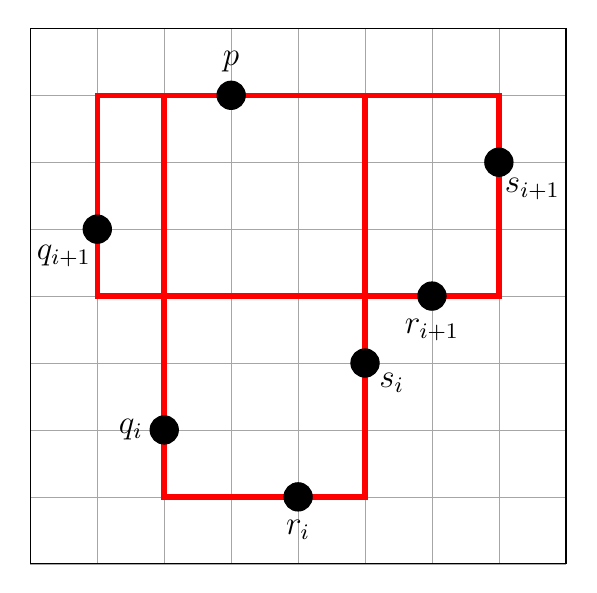
\begin{tikzpicture}[scale=0.85]
            % Grade de fundo
            \draw[very thin, gray!70] (0,0) grid (8,8);  
            \draw[red,line width=0.07cm] (2,1) rectangle (5,7);
            \draw[red,line width=0.07cm] (1,4) rectangle (7,7);

            \node at (4,0.5) {\textbf{\large $r_i$}};
            \node at (1.5,2) {\textbf{\large $q_i$}};
            \node at (5.4,2.7) {\textbf{\large $s_i$}};
            \node at (6,3.5) {\textbf{\large $r_{i + 1}$}};
            \node at (0.5,4.6) {\textbf{\large $q_{i + 1}$}};
            \node at (7.5,5.6) {\textbf{\large $s_{i + 1}$}};
            \node at (3,7.5) {\textbf{\large $p$}};
            %\node at (4.4,3.3) {\textbf{\large $a_j$}};
            %\node at (2,4.5) {\textbf{\large $p$}};
            
            % Pontos
            \filldraw[black] (4,1) circle (6pt); %ai
            \filldraw[black] (2,2) circle (6pt); %ai+1
            \filldraw[black] (5,3) circle (6pt); %aj
            \filldraw[black] (6,4) circle (6pt); %p
            \filldraw[black] (1,5) circle (6pt); %p
            \filldraw[black] (7,6) circle (6pt); %p
            \filldraw[black] (3,7) circle (6pt); %p
            
            % Limite do quadrado
            \draw[black, line width=0.5pt] (0,0) rectangle (8,8);
        \end{tikzpicture}
    \caption{Estão ilustrados dois z-retângulos consecutivos formados por $p$ e pontos de seu funil em~$P$. Note que $s_i$ e $r_{i+1}$ podem ser rótulos de um mesmo ponto de $P$.}
    \label{fig:funil-2-z-rets}
    \end{figure}
\end{proof}

\begin{corollary} \label{corollario:final} %COROLÁRIO!!!
    Para qualquer sequência $X$ de acessos, $\Funil(P_X) \geq \Funil(\widebar{P_X}) - \Theta(m)$.
\end{corollary}

\begin{proof}
    \begin{align*}
        \Funil(P_X) &\geq 2 \cdot zRet(P_X) \quad & \text{pelo Lema~\ref{lemma:funil-zrets}}, \\
        &= 2 \cdot zRet(P_X^{\perp}) \quad & \text{pelo Lema~\ref{lemma:p-inversivel}}, \\
        &= 2 \cdot zRet(P_X^{\perp\perp}) \quad & \text{novamente pelo Lema~\ref{lemma:p-inversivel}}, \\
        &= 2 \cdot zRet(\widebar{P_X}), \\
        &\geq \Funil(\widebar{P_X}) - \Theta(m) \quad & \text{pelo Lema~\ref{lemma:zrets-funil}}. \\
    \end{align*}
\end{proof}

\begin{theorem}
    Para toda sequência $X$ de acessos sem repetições e para toda árvore de referência $\cT$ em relação a $P_X$, $\Alt(P_X) \leq \Oh(\Funil(P_X) + m)$.
\end{theorem}

\begin{proof}
    \begin{align*}
        \Alt_{\cT}(P_X) &\leq \Funil(P_X) +  \Funil(\widebar{P_X}) \quad & \text{pelo Lema~\ref{lemma:relacao-alt-com-funil}}, \\
        &\leq \Funil(P_X) +  \Funil(P_X) + \Theta(m) \quad & \text{pelo Corolário~\ref{corollario:final}}, \\
        &= \Oh(\Funil(P_X) + m).
    \end{align*}
\end{proof}

Esses resultados são bastante impressionantes dado que delimitações construídas a partir de z-retângulos são invariantes em relação a rotações. Além disso, os z-retângulos nos mostram que rotações dos conjuntos de pontos de visões geométricas de sequência de acessos têm seu custo relacionado, ou seja, a grosso modo, fazer $m$ buscas no conjunto de chaves de $1$ a $n$ tem seu custo relacionado com inverter os eixos e fazer as $n$ buscas correspondentes no conjunto de chaves de $1$ a $m$. Esse resultado é fascinante. 
